\documentclass[12pt]{article}
\bibliographystyle{plainurl}
\usepackage{graphicx}
\usepackage[margin=1in]{geometry} % sets margin size
\usepackage{indentfirst}
\usepackage[section]{placeins} % prevents figures from separating from their sections
\usepackage{hyperref}
\title{System Communication: Real-Time Data Transport Prototype}
\author{L. Callahan, N. DePergola, A. Kaufmann,\\D. Lalli, T. Matson, T. Nguyen}
\date{October 2026}
% Defining the document setup and imports above
% Use the percent sign to make comments in LaTeX

\begin{document}
\maketitle % importing the title we defined above.

% Adding this line break === between sections for clarity
%=====================================================================================

\section*{Abstract}

\textbf{Ultimate goal of why we built this prototype: to explore feasible design options for ngRadar inter-site data communication, so that the project can make informed architectural decisions about public-network data movement, remote observing, and real-time feedback between GBO, VLBA sites, DSOC, and observers or operators. Also to create a system that could be used in other areas of the observatory, outside just the context of ngRadar}

Interferometers used in Radio Astronomy require real time communication between antenna sites and new instruments, such as the ngVLA, and ngRadar would strongly benefit from system communication between observation planning, telescope control, and data transport software. Currently, there is no direct connection between these software components and NRAO personel must communicate directly to plan observations across sites.
This software documents a real-time data transport architecture developed by the NRAO, and demonstrates a possible use in the future ngRadar system, but could be implemented into any radio astronomy observatory. The software architecture is entirely event-driven while each event is also saved in a central database, with every event visible to users on a public website. The prototype has been tested with simulated observation data, and has demonstrated the ability to work remotely across geographically dispersed sites. 

%=====================================================================================

\section{Introduction} \label{Introduction}

\textbf{Note from Nicole: I want it to be clear that yes, our prototype was devleoped in the context of ngRadar, so we will stick with that terminology, BUT the goal of this prototyping cohort was to investigate tools that could be used for several projects at NRAO.}
The ngRadar system will utilize the Green Bank Telescope as a high powered transmitter, capable of transmitting a 13.7 GHz frequency at 500kW, and be able to image objects 10 times farther than the lunar distance. The Very Long Baseline Array (VLBA) will be used to receive those signals, before being sent to the Domenici Science Operations Center (DSOC) for data processing. During test observations with the low powered transmitter, scientific staff had to communicate over the phone with telescope operators across the GBT and VLBA sites to coordinate planned observations, including observation targets and times.

  The Real-Time System Communication Prototype was developed to demonstrate system communications between remote NRAO locations. This paper documents an event-driven, web-based application for remote viewing of an active observation across geographically dispersed sites. Although this software could be implemented on many NRAO observatories, the ngRadar system was chosen for our team to demonstrate the prototype's proof of concept.

This memo details the software system architecture (Section \ref{System Architecture}), design decisions (Section \ref{Design Decisions}), software components and technologies chosen (Section \ref{Software Stack}), and other dependencies required by the System Communication Prototype (Section \ref{Dependencies}). \textbf{Needs Laura's stamp of approval.}

%=====================================================================================

\section{System Architecture} \label{System Architecture}

  To enable system communication across NRAO sites, the software may need to be compatible with various types of machines and operating systems. For use in ngRadar, the software would need to communicate across the continental United States, Hawaii, and the Caribbean.
    
  The team initially investigated developing software which would be installed locally on the computers of NRAO employees, and transmit data over the internet to the software at other locations. However, this would have required compiling and building an application for all three major operating systems. Therefore, it was decided that the software would not be locally hosted, and instead function as a web application. This website would be primarily hosted on servers at DSOC, with other software components hosted at the Green Bank Observatory and on all 10 of the VLBA sites. 

  While Apache Kafka is responsible for sending and receiving event notifiers on the website, another software tool must be used to send the actual observation data from the receiving antennas to DSOC. The team investigated two different tools for the movement of observation data. The first tool demonstrated with this software is E-transfer, an open source client/daemon used for high speed data transfers and developed by the Joint Institute for Very Long Baseline Interferometry European Research Infrastructure Consortium (JIVE). Additionally, the team demonstrated ExpeDat, a data transfer tool which utilizes a proprietary file transport protocol based on UDP. ExpeDat was developed by Data Expedition inc, and the software is available as a free trial or for purchase with a one time fee. Due to project time contraints, the team spent 8 weeks using E-transfer for transmitting observation data, but only 2 weeks using ExpeDat. However, data collected on the performance of these tools showed \textbf{[fill in later]} consistently worked faster.
  
  This web application did not make use of a dedicated front-end framework, and instead used HTML pages supported by Javascript, CSS, and bootstrap code. To store and display information generated by the simulated observation events, an SQL database was used. PostgreSQL was chosen because it is open source, free, and widely used across tech companies. The database is hosted at the simulated DSOC location within our software prototype. It should be noted that while the database is responsible for storing the history of observed events, the database is not required for the website to function, as it is entirely driven by Kafka message events.

  Security was an important consideration during the development process - if a web application with similar design architecture is implemented for actual use in ngRadar, it will run directly on NRAO computers across numerous observatory locations, and potentially interface with telescope hardware. Docker Containers play a role in keeping local computers safe, since applications within them are isolated from the rest of the computer. Django also has several built in security features, including user authentication, cross site scripting, and forgery attack protection.

  During the development process, the team needed a way to ensure that this website could be run across multiple machines for local development and debugging, but also perform reliably when run on a cloud-based or locally hosted server. To accomplish this, we used Docker Containers to isolate software components and their dependencies used on our website. This would ensure that any computer which has the Docker Engine - a server responsible for managing the containers - can run this web application and it will perform consistently.
  
  Fig. \ref{fig:step1} shows the first step of the system sequencing. The user submitting a new waveform indicates the beginning of the process, which triggers the initial Kafka message. An arrow from A to B represents a Kafka message produced by A and consumed by B. 

\begin{figure}[h!] 
\centering 
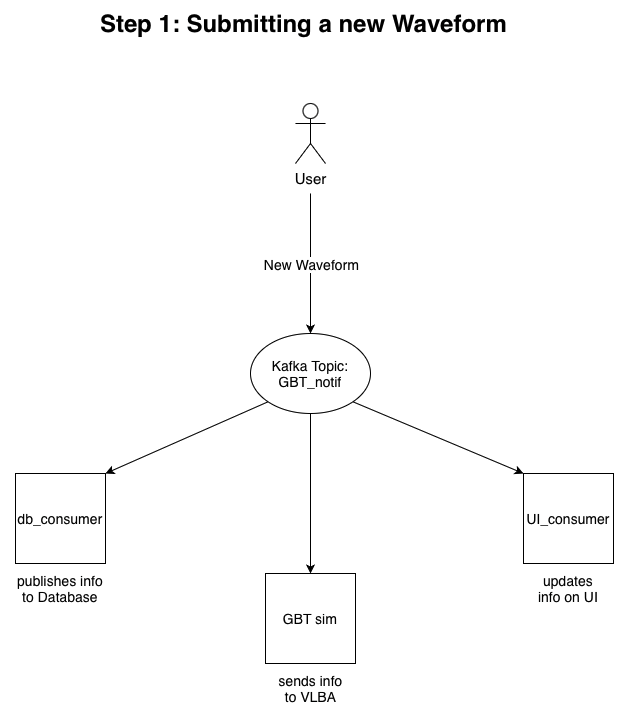
\includegraphics[width=0.65\columnwidth]{figures/Step1_sequence.png} 
    \caption{*\textbf{Note for team}: the quality of this image is bad. We can replace it once we agree if we want to use it!} 
    \label{fig:step1}
\end{figure}

\begin{figure}[h!] 
\centering 
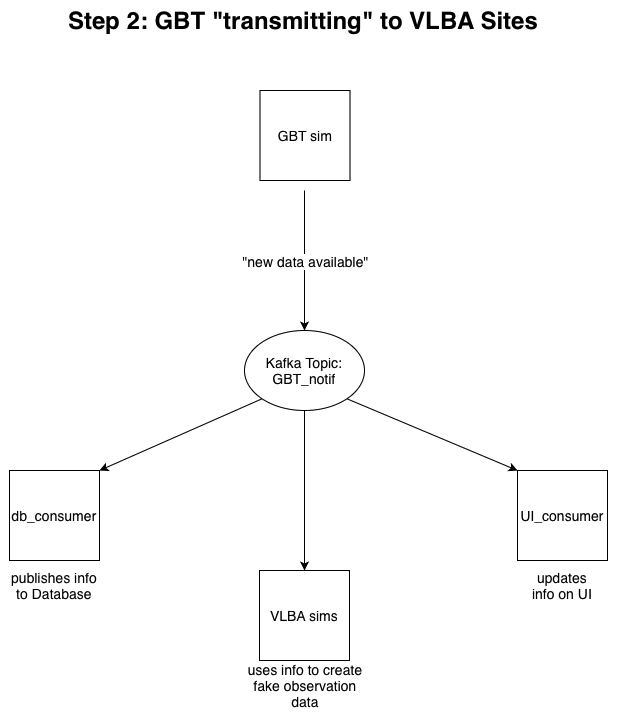
\includegraphics[width=0.65\columnwidth]{figures/Step2_sequence.png} 
    \caption{*\textbf{Note for team}: the quality of this image is bad. We can replace it once we agree if we want to use it!} 
    \label{fig:step2}
\end{figure}

\begin{figure}[h!] 
\centering 
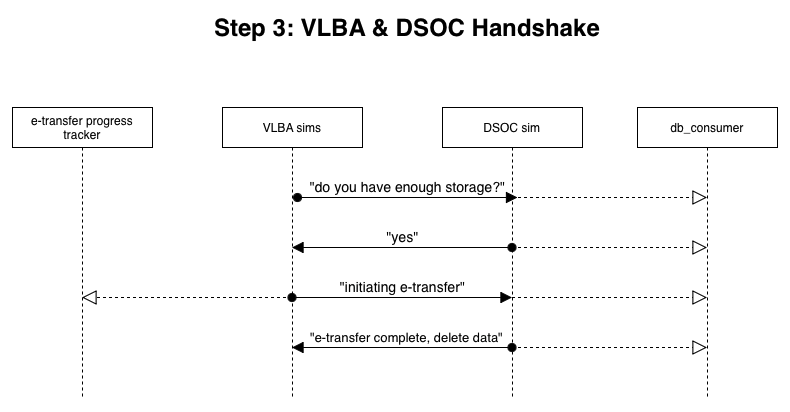
\includegraphics[width=0.65\columnwidth]{figures/Step3_sequence.png} 
    \caption{*\textbf{Note for team}: the quality of this image is bad. We can replace it once we agree if we want to use it!} 
    \label{fig:step3}
\end{figure}

%=====================================================================================

\section{Design Decisions} \label{Design Decisions}

\subsection*{Desktop Application versus Web Application}
  To enable system communication across NRAO sites, the software needs to be compatible with various types of machines and operating systems. For use in ngRadar, the software would need to communicate across the continental United States, Hawaii, and the Caribbean.
    
  The team initially investigated developing software which would be installed locally on the computers of NRAO employees, and transmit data over the internet to the software at other locations. However, this would have required compiling and building an application for all three major operating systems. Therefore, it was decided that the software would not be locally hosted, and instead function as a web application. This website would be primarily hosted on servers at DSOC, with other software components hosted at the Green Bank Observatory and on all 10 of the VLBA sites. 

\subsection*{Backend Frameworks}

There were three frameworks our team investigated - Flask, FastAPI, and Django.
  Flask is well-known for its simplicity and low usage of computing resources. It is also flexible and modular, allowing developers to modify the framework and integrate additional software components for added functionality. However, Flask only supports using synchronous communication between the server and framework, meaning processes can only run one-at-a-time. Flask also does not have built in authentication or adminstrative features.

  FastAPI provides high-speed, and asynchronous, non-blocking communication in a relatively lightweight framework. It is the newest framework we investigated and includes features such as built in authentication, python code completion to speed up development, and automatic documentation for program APIs. It includes a modest number of built in functionality, and developers can add libraries with additional features they need.

  Django is a framework with a large amount of built in functionality including an adminstrative dashboard, user authentication, HTML form processing, and an object-relational mapper for database interaction [\textbf{Revisit and add any additional built-in features we used}]. It is capable of running large web applications with many users. By default, Django runs with synchronous communication, but libraries that add asynchronous communication are avaliable.

  After considering all three frameworks, Django was chosen due to the large number of compatible software libraries, built in security and adminstrative features, and its ability to scale as website traffic grows.


\subsection*{Event Orchestrators}

  Real time data transmission across geographically separated locations was a defining requirement of our software prototype, and choosing a software tool to accomplish this was a major decision the team needed to make early in the design process. Initially, the team was considering using Socket programming for communication over the internet, but the added complexity of developing our own code to do this reliably with multiple computers led us to investigate using an existing message broker to accomplish this.

There were three message brokers the team investigated using - Apache Kafka, RabbitMQ, and Apache Pulsar. Apache Kafka was first released to the public in 2011, and is the most widely used message broker across the industry. It is best suited for high volume data transmission, and uses a central server known as a cluster, with one or more message brokers to handle requests from producers and consumers. Kafka uses "producers" to send messages to user-defined topics. Messages are stored in these topics in subgroups called partitions, either until consumption is confirmed or for a fixed number of days. "Consumers" are used to receive messages from these topics. The initial time to implement a basic Kafka messaging setup was minimal; however, scaling up the system and debugging errors adds significant complexity. Kafka can also use more computing resources than necessary if only sending a small amount of data. However, Kafka is very reliable, and has several built in methods to prevent data loss if servers crash. 

RabbitMQ was also considered as a broker option; it has the lowest message latency and lowest server memory requirement compared to the other two options, and is a significantly simpler system. This option was not chosen due to RabbitMQ's push model (producer controls the flow of messages and can overwhelm consumers) and the difficulty in scaling up the system. Apache Pulsar, the third option considered, is the newest of the three message brokers and attempts to combine the features of Kafka and RabbitMQ. Pulsar is well suited for scaling up to handle high volumes of data. However, with the extra features Pulsar offers, it is more complex to setup than Kafka, has a higher message latency due to the extra storage layers, and has less documentation avaliable.

  Ultimately the team decided to select Kafka, as it has many highlights: extensive use across the industry, high reliability and customization when sending or receiving messages, and the large amount of documentation avaliable for it. One of the most important features of Kafka for our prototype is the publish/subscribe model, and the ability for multiple consumers to retrieve information from a single producer. 
  
  Kafka has numerous options for online broker hosting, and initially the website was set up to work with Confluent Cloud. However, the team chose locally hosted Kafka brokers due to lower cost, increased flexibility, and more control over the data on those brokers.

\subsection*{SQL Database}

\subsection*{File Store}

This software prototype simulates generating DDM images from the VLBA Antenna stations, and storing these images directly in a database as binary files significantly reduces performance and increases database size when large numbers of images need to be produced. Using a dedicated File Store means the database only needs to store text-based information, enabling faster database queries and the ability to serve images using SDKs such as Amazon Boto3. 

\subsection*{Data Movement}

  Etransfer is the first data transfer tool tested within this prototype, which was developed by the Joint Institute for VLBI ERIC (JIVE) and has become the standard data transfer tool within the VLBI community. The code repository for this tool is free to use and open source, which benefits development by allowing us to adjust the code as needed \cite{marjolein_verkouter_jive-vlbietransfer_2026}. Etransfer supports TCP, UDT, and SRT, with UDT and SRT being the recommended protocols. The etransfer client (etc) and etransfer daemon (etd) system allows the client program to initiate both client to server transfer, as well as server to server transfers, during which the data does not flow through the client's machine and/or network (note that server and daemon are interchangeable). This tool supports resuming failed transfers, mutliple transfers to one daemon in parallel, and Access Control Lists to define allowed/denied directories. It does not yet support authentication and authorization.

\url{https://nrao.atlassian.net/wiki/x/GQBoRw}

\url{https://nrao.atlassian.net/wiki/x/AQDRS}

\url{https://nrao.atlassian.net/wiki/x/AQAZSg}

\url{https://nrao.atlassian.net/wiki/x/HABRV}

  ExpeDat is the second data transfer tool the team evaluated for use in this website, and it was developed by Data Expedition Incorporated. Unlike most of the other code in this prototype, it is proprietary and uses the Multipurpose Transcation Protocol (MTP), a data transport protocol which can adapt to changes in network conditions, and is based on the open source User Datagram Protocol (UDP). The software consists of a server and several client applications to move files between networked computers. It is capable of resuming incomplete file transfers, compressing data before transferring it, tracking file upload status, and remotely monitoring the server status. These settings can be changed in the \textit{servedat.cf} and \textit{svpasswd} files. The client and server can be set up and installed on Windows, Linux, and MacOS, or configured to run inside a docker container.


\subsection*{Cloud-Hosting Solutions}

  While developing this website, the team needed a way to test our simulation code from geographically distributed locations, to simulate how a similar software architecture would be implemented if used with ngRadar where our cloud-hosted website could inform a remote viewer of real-time events during an activer observation.
  
  One cloud-hosting platform the team considered was Render....
  
  Ultimately, the team decided to use Digital Ocean as the cloud-hosting solution because....
  
  In a version actually used with telescope hardware, this website would be hosted using NRAO servers on site, but for this prototype, the team used DigitalOcean, a cloud hosting platform, which sells access to run code on Virtual Machines, known as "Droplets" at various locations worldwide. The team set up Droplets on servers located in New York, San Francisco, London, Bangalore, and Sydney to run our website containers. Digital Ocean offers Droplets with varying performance levels, and our team purchased monthly subscriptions to four entry level droplets, and one mid-tier droplet. Each entry level Droplet offered 1 virtual CPU (vCPU), 2GB of RAM, 50GB of storage, and costs \$12 per month. The mid tier droplet has 4 vCPUs, 8GB of RAM, 160GB of storage, and costs \$48 per month. The portion of our website representing DSOC contains the software tools which managed the SQL database, Kafka brokers, E-transfer (or ExpeDat) server, SeaweedFS file store, and various performance monitoring tools. To perform at an acceptable speed and support multiple website users, the team found that DSOC needed to use this mid-tier droplet. The other portions of our website, including the GBT and VLBA simulators, were spread out evenly across the 5 Droplets.
\url{https://nrao.atlassian.net/wiki/x/BoDsT}

\url{https://nrao.atlassian.net/wiki/x/BACsTg}

\url{https://nrao.atlassian.net/wiki/x/AYAqUg}



%=====================================================================================

\section{Software Stack} \label{Software Stack}

\subsection*{Django-Based Web Application}

  Since we were building a prototype and not concerned with computing speed or processing power, we chose Python as our backend language, with Django as our backend framework since it's a robust and feature-rich framework for building a website application quickly. Throughout the development of the prototype, a front-end framework was never selected as Django's Models Views Templates (MVC) was sufficient for the needs of the website. Our frontend is comprised of html, css, and javascript. 


\subsection*{Docker Containerization}

  The team decided to containerize all backend components and technologies used in this System Communication Prototype using Docker, resulting in approximately 32 containers. We spun up all 32 containers during local development, and also when hosted on the Digital Ocean Droplets on the cloud, with droplets being hosted in data centers in geographically dispersed regions around the world. 
  gbt, dsoc, 10 vlbas, progress_tracker, db_consumer, ui_consumer (runs in a single thread spun up inside the website container), dsoc-volume-init, expedat_server, postgres_exporter, kafka_exporter.
  Shared volumnes when necessary, shared Docker DNS network bridge - used both locally and when hosted on the DO Droplets. 
  For this simulation, we had 1 cloud-hosted droplet based in a San Francisco data center which hosted our gbt_sim container, 2 vlba_sim containers, a portainer agent, and a kafka node. We had 1 droplet based in London with 2 vlba sim containers, a portainer agent, and a kafka node. We had 1 droplet based in Bangalore with 2 vlba sims and a portainer agent. We had 1 droplet based in Sydney with 2 vlba sims and a portainer agent. We had 1 droplet based in New York which hosted our dsoc sim, 2 vlba sims, our public facing website, seaweedfs, kafka, posgres database, a central portainer which all portainer agents send their health status to, traefik for routing public internet traffic to and from the docker DNS on the droplets, prometheus, opentelemetry, and grafana. 

\subsection*{Digital Ocean Droplets}
  Droplets: 

\subsection*{Apache Kafka Event Messenger}

  kafka-init (used to create our kafka topics if they have not been created before, such as after doing a hard-reset of our local environment, or deploying our kafka nodes to a new machine for the first time), multi-node kafka cluster (1 kRaft controller node, 2 follower nodes) kafka_ui. 4 kafka topics: gbt_notif, vlba_notif, dsoc_notif, progress_tracking (for vlba progress updates of its expedat streaming that the ui_consumer will consume and SSE update the UI progress bars)
  Our gbt sim, vlba sims, dsoc sim, ui_consumer, and db_consumer all consume kafka event messages. The submit waveform button on our UI publishes a kafka message to the gbt_notif kafka topic, which the gbt sim is subscribed to, to notify the gbt sim that a user has selected a new waveform and so the gbt sim can begin transmitting based on that new waveform. The gbt sim will send a kafka message back to the gbt_notif which the ui_consumer is subscribed to and will update the UI via Server Side Events (SSE) to notify the user that the GBT has started transmitting that new waveform. The vlba sim is subscribed to the gbt_notif as well, and will listen for an explicit kafka message indicating a change in waveform (ignoring all other gbt_notif messages) before proceeding with the rest of the vlba simulated workflow steps. The vlba sim published to the vlba_notif kafka topic which the dsoc_sim is subscribed to. These kafka events initiate logical workflow steps between the vlba sim and the dsoc sim; workflow steps like the vlba sim requesting to stream its raw data to a shared directory that dsoc owns, dsoc performing a storage check and responding yes or no, vlba streams data to dsoc and dsoc validates the expected size of data with the actual size of data it received. After which, dsoc produces kafka messages to the dsoc_notif topic for the following events: generates a fake DDM image, stores the DDM in seaweedfs, notifies the vlba sim stations that they may delete their raw data, and publishes 'Complete', indicating the end of the simulated observation. 
  The db_consumer and the ui_consumer are also subscribed to all 4 kafka topics. The ui_consumer is responsible for consuming events from the 4 topics and via Server Side Events, update the UI's home page immediately. The db_consumer is also subscribed to all 4 kafka topics and it is responsible for consuming all events, inserting a new record in a master postgres database table for historical persistence of the simulated observation, then SSE updating the UI's history events page. This means that the home page is completely decoupled from a database, instead it relies on kafka for orchestrating its real-time simulated observation events. 
  We created a templated kafka payload that remains consistent throughout the entire sequencing of events and which gets updated with new metadata that the next step in the sequence will need in order to do its processing. When done, it fills out the kafka template with more data that the next step in the sequence will need to proceed with its sequencing. In total, the kafka metadata that kafka sends from step to step is quite small, about 



\subsection*{PostgreSQL Database}



\subsection*{ExpeDat Streaming}


\subsection*{SeaweedFS - Object Store}

SeaweedFS is an open source tool that can function as both an object store and a file store. For the purposes of this prototype, we only explored using Seaweedfs as an object store, rather than a file store, but it does support both. 

\subsubsection*{Traefik}

  Traefik is a modern, open-source reverse proxy and load balancer used to route incoming network traffic to the correct backend services. Traefik integrates seamlessly with Docker, automatically discovering new services on the Docker DNS. Traefik also integrates with Let’s Encrypt to automatically generate, manage, and renew SSL/TLS certificates for secure web traffic. For these reasons, the team chose to adopt Traefik to handle exposing the ngRadar website from a Docker container to a public IP address.


\subsection*{Performace \& Monitoring Tools}

Portainer + Portainer Agents, Prometheus, Grafana, k6, OpenTelemetry and Tempo, 

\subsubsection*{Portainer + Portainer Agents}

\subsubsection*{Prometheus}

\subsubsection*{k6}

\subsubsection*{OpenTelemetry and Tempo}

\subsubsection*{Grafana}



%=====================================================================================

\section{Dependencies} \label{Dependencies}

%=====================================================================================


\section{Ideas for Future Improvements} \label{Future}
%===== Some of these may be resolved in [760] Final Technical Cleanup? Not sure

\begin{itemize}
  \item Features
  \begin{itemize}
    
    \item Originally, DSOC checks its storage and responds to a single VLBA station if it can accept the incoming e-transfer/expedat raw data transfer/stream. Currently, we have this check occurring simultaneously for all 10 VLBA stations. But we noticed that with 10 consecutive storage check requests, DSOC responds yes without taking into account the requests it’s already approved. With the simultaneous transfers/streams, DSOC storage could potentially go over its storage limit for incoming raw data. It would be beneficial to have some logic built in place for DSOC to keep track of its storage before and after each approval of a requested VLBA site's incoming transfer/stream.
    
    \item Currently, on our history events page, you can see that in our sequencing of events, DSOC sends a 'Completed' kafka message 10 times per 10 VLBA sims. It might make more sense to have DSOC wait until it has finished processing all 10 VLBAs raw data, generates its 10 DDM images and stores them to seaweedfs, and then send only one 'Completed' kafka message to be displayed on the UI and communicate to the remote observer that the sequencing of events has finished. 
  
  \end{itemize}
  
  \item Known issues
  \begin{itemize}
    
    \item The submit new waveform button currently unlocks after the first of several concurrent VLBA transfers completes, rather than after all of them have completed.
    \item Part way through the prototype's development we had a big refactor to decouple our UI from the postgres database and convert the UI to be completely event-driven by relying on kafka for updates to the UI rather than polling the database to update the UI. Before this refactor, we had built certain safeguards to ensure that the website, backend processes, and our docker ecosystem could fail gracefully and print helpful logs for debugging and restarting, rather than failing and exiting. We have not tested any of the graceful failure scenarious since the UI Bridge refactor, so it would be valuable to go back through those scenarious and ensure that the prototype fails gracefully. 

  \end{itemize}
\end{itemize}

%=====================================================================================
\bibliography{zotero-dmspc-technical-memo}

\end{document}
